\documentclass[pra,superscriptaddress,groupedaddress,twocolumn]{revtex4}
\usepackage{graphicx}  % needed for figures
\usepackage{siunitx}   % for decimal alignment in tables
\usepackage{bm,amssymb,amsmath}    % for math
\usepackage[bookmarks]{hyperref}
\usepackage{threeparttable}

\begin{document}

\title{How Large are Non-adiabatic Effects in Realistic Systems?}
\input{Section/authors}
\begin{abstract}
In this work we calculate the non-relativistic ground-state energies of atomic and molecular systems with and without the Born-Oppenheimer approximation. For this we utilize the fixed-node diffusion Monte Carlo method, in which the nodes depend on both the electronic and ionic positions. We report ground-state energies, ionization energies and atomization energies to a statistical accuracy of less than $0.1$ mHa for all but the largest systems. We find the ionization energies of the atoms to be independent of the adiabatic assumption except for O and F where the non-adiabatic and clamped-ion ionization energies differ by less than 0.5 mHa. The atomization energies, however, are influenced by the non-adiabatic coupling between electrons and nuclei at the mHa level. We demonstrate that the fixed-node approximation provides a highly accurate and scalable approach to treating molecular systems beyond the Born-Oppenheimer approximation.
% This observation suggests that the non-adiabatic coupling between the valence electrons and nucleus motion is not important in the ionization process.
\end{abstract}
\maketitle

\section{Introduction}
There have been several recent discoveries~\cite{cederbaum1,gross2014,boent} suggesting that quantum wave functions, which include both electronic and ionic degrees of freedom, have many interesting properties that have yet to be explored.  This includes the development of equations that exactly factorize a wave function into electronic and ionic components~\cite{cederbaum1}, the disappearance of conical intersections in wave functions of model systems~\cite{gross2014}, and the use of quantum entanglement to study electronic and ionic density matrices~\cite{boent}.  Extending such studies to realistic systems is of broad interest and will considerably expand our understanding of electron-ion systems. However, treatment of \textit{ab initio} electron-ion systems is challenging, and applications have thus been limited. The most accurate simulations of electron-ion wave functions are generally done with very specialized wave functions, which are limited to rather small systems \cite{mitroy2013}.  

As a framework to address these problems in general realistic systems, we recently demonstrated that quantum Monte Carlo (QMC) can be combined with quantum chemistry techniques to generate electron-ion wave functions~\cite{Tubman_ECG}.  We treated realistic molecular systems and demonstrated that our method can be scaled to larger systems than previously considered while maintaining a highly accurate wave function. In the following we extend our previous work by considering the simulation of a larger benchmark set of atoms and molecules.  We calculate ionization energies and atomization energies that can be directly compared with previous benchmarking results.

Adhering to the definitions given by Worth and Cederbaum \cite{Cederbaum_Review},
Born-Oppenheimer (BO) assumption will refer to the approximation of the full electron-ion wave function by a single product of an ionic wave function and an eigenstate of the electronic Hamiltonian. The adiabatic approximation will refer to the further neglegence of the diagonal Born-Oppenheimer correction (DBOC) term in solving for the ionic wave function. In this context, the clamped-nuclei ground-state energy $E_c$ is the lowest eigenvalue of the electronic Hamiltonian and the non-adiabatic ground-state energy $E_n$ is the eigenvalue of the full molecular Hamiltonian. %The BO energy is the sum of the clamped-nuclei energy and zero-point energy (ZPE) of the nuclei estimated without the DBOC term whereas the adiabatic energy includes ZPE with the DBOC term.

\section{Method}
\subsection{Fixed-Node Diffusion Monte Carlo (FN-DMC)}
Diffusion Monte Carlo is a projector method that evolves a trial wave function in imaginary time and projects out the ground-state wave function.  For practical simulations of fermions, the fixed-node approximation is introduced, which depends only on the set of electronic positions where a trial wave functions is equal to zero.  This approximation is different than approximations typically used in quantum chemistry calculations, and in this work we demonstrate that we can generate high quality nodal surfaces for a range of systems that include full electron-ion wave functions. 

If the trial wave function has the same nodal surface as the exact ground-state wave function, FN-DMC will obtain the exact ground-state energy.  Approximate nodal surfaces can be generated through optimization of the full wave function. Such approximate nodal surfaces have been tested and validated on a wide range of systems, and consistently provide an excellent approximation of the exact ground-state energy,  comparable to the state of the art in \textit{ab initio} simulations~\cite{grossman1}. In addition, the energies generated with FN-DMC are variational with respect to the ground-state energy.

In all but a handful of previous QMC simulations, calculations are performed with the electronic Hamiltonian alone (with nuclei "clamped" to their equilibrium positions). Recent advances~\cite{Nightingale_Linear,Umrigar_Linear,Brown_Bench} have made it possible to optimize thousands of wave function parameters simultaneously with variational Monte Carlo within the clamped-nuclei approximation. However, such an assumption is not fundamentally required by FN-DMC. In our previous work we find that the most important effects for optimizing are the nodes due to electron-electron correlation~\cite{Tubman_ECG}, and in this regard we use more sophisticated terms in the electronic part of the wave function than in the ionic part.

\subsection{Electronic Wave Function and Optimization}

There are several different approaches for generating high quality electronic wave functions for a FN-DMC calculation~\cite{Umrigar_Alleviation,Toulouse_Bench,Brown_Bench,Seth_Bench}. We use an initial guess for the wave function that is generated from complete active space self-consistent-field (CASSCF) \cite{Chaban_MCSCF,Szabo} calculations using the quantum chemistry package GAMESS \cite{GAMESS}. The optimized orbitals are then used in a configuration interaction singles and doubles (CISD) calculation to generate a series of configuration state functions (CSF)~\cite{Clark_Bench}. For LiH and BeH, a CASSCF calculation with a large active space is used in place of CISD. The multi-CSF expansion of the wave function can be expressed in the following form,
\begin{align}
\Psi_{\text{CISD}}(\vec{r};\vec{R}_o)=\sum\limits_{i=1}^{N_{\text{CSF}}}\alpha_i\phi_i(\vec{r};\vec{R}_o), \label{eq:psi_gms}
\end{align}
where $\vec{r}$ refers to the spatial coordinates of all the electrons and $\vec{R}_o$ refers to the equilibrium positions of all the ions. $\phi_i(\vec{r})$ and $\vec{\alpha}=\{\alpha_1,\alpha_2,\dots\}$ are the CSF and CI coefficients generated from CISD. The cc-pV5Z basis \cite{dunning} is used for the atomic systems and Roos Augmented Triple Zeta ANO basis~\cite{roos} for the molecular systems except for the smallest system LiH where the cc-pV5Z basis is used.

After the multi-CSF expansion is generated, we impose the electron-nucleus cusp condition on each molecular orbital~\cite{cusp} and add a Jastrow factor to the wave function to include electron correlation~\cite{Kato}. Our Jastrow factor contains electron-electron, electron-nucleus and electron-electron-nucleus terms. The full electronic wave function used in FN-DMC is then,
\begin{align}
\psi_e(\vec{r};\vec{R})=e^{J(\vec{r},\vec{R},\vec{\beta})}\Psi_{\text{CISD}}(\vec{r};\vec{R})\label{eq:psie}
\end{align}
We optimize the CSF and Jastrow coefficients $\vec{\alpha},\vec{\beta}$ simultaneously with QMCPACK \cite{QMCPACK}. Optimization is performed with the ions clamped to their equilibrium positions. We include all CSFs with coefficients lager than a specific cutoff $\epsilon$ to lend reasonable flexibility to the wave function during optimization. We include as many CSFs as possible to maximize the flexibility of the wave function. However, the inclusion of too many CSFs with small expansion coefficients can introduce noise as they require a large number of samples in the optimization step to be optimized. We have chosen $\epsilon$ to restrict the number of CSFs in the wave function to be $\sim$1000 in all systems. Optimization was performed with the linear method with roughly $10^6$ statistically independent samples, and we use a cost function consisting of equal parts average local energy and reweighted variance.

\begin{figure}[h]
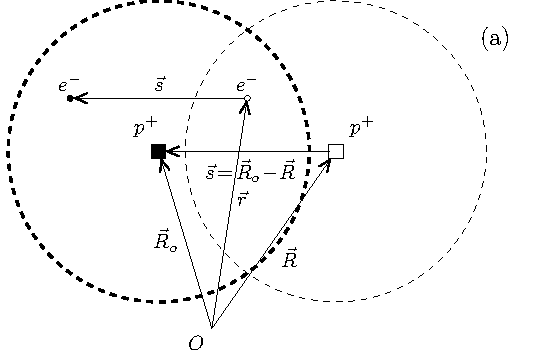
\includegraphics[width=9cm]{fig1a.pdf}
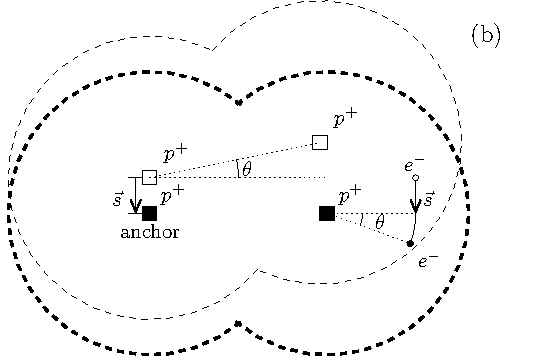
\includegraphics[width=9cm]{fig1b.pdf}
\caption{ Symmetries for simulation of atomic and molecular systems in QMC {\bf (a)} For atomic systems we can consider the entire wave function shifting with the ion. This process can be visualized by following a contour of the wave function. The thick dashed circle represents a contour of the electronic wave function when the proton is at its reference position $\vec{R}_o$ and the thin dashed circle represents the same contour when the proton has moved to a new position $\vec{R}$. To evaluate the ion-dependent electronic wave function $\bar{\psi}_e(\vec{r},\vec{R})$, we simply map the electron to its proper place in the reference wave function $\psi_e(\vec{r};\vec{R}_o)$. That is, $\bar{\psi}_e(\vec{r},\vec{R})=\bar{\psi}_e(\vec{r}+\vec{s},\vec{R}_o)=\psi_e(\vec{r}+\vec{s};\vec{R}_o)$ where $\vec{s}$ is the shift required to put the proton back to its reference position. {\bf (b)} For H$_2^+$, we pick one of the protons as an "anchor" and approximate the new wave function by dragging the reference wave function with the "anchor" proton. We also rotate the wave function to align its axis of symmetry with the orientation of the two protons. \label{fig:drag}}
\end{figure}

\subsection{Electron-Ion Wave Function}

Once a satisfactory electronic wave function has been obtained, we construct the electron-ion wave function using the ansatz previously investigated~\cite{Tubman_ECG},
\begin{align}
\Psi_{eI}(\vec{r},\vec{R})=\psi_I(\vec{R})\bar{\psi}_e(\vec{r},\vec{R}), \label{eq:psi}
\end{align}
where $\vec{R}$ denotes the spatial coordinates of all ions and $\bar{\psi}_e(\vec{r},\vec{R})$ is an ion-dependent electronic wave function adapted from the clamped-ion wave function $\psi_e(\vec{r};\vec{R}_o)$ through basis set dependence. Due to the nuclear localization of the Gaussian electronic basis set used in the quantum chemistry calculations for constructing the electronic wave function, the nodes of $\bar{\psi}_e$ change based on the ionic positions, which we have previously called the dragged-node approximation~\cite{Tubman_ECG}. In general, the nodes only coincide with those obtained in the clamped-ion limit when the ions are at their equilibrium positions $\bar{\psi}_e(\vec{r},\vec{R}_o)=\psi_e(\vec{r};\vec{R}_o)$. However, for atoms and ions this approximation is equivalent to re-optimizing the electronic wave function at each ionic configuration, i.e. $\bar{\psi}_e(\vec{r},\vec{R})=\psi_e(\vec{r};\vec{R})$. Although there are approaches for going beyond the dragged-node approximation, it was demonstrated to be highly accurate over a range of molecules in previous work.~\cite{Tubman_ECG} For the systems considered here, we can impose various symmetries of the Hamiltonian onto the wave function that arise from the relative motion of the ions. In Fig.~\ref{fig:drag} we demonstrate this strategy for the simple cases of a hydrogen atom and a H$_2^+$ molecular ion. This can be generalized for use in larger systems or even applied to parts of a bigger system, e.g., treating light ions as quantum particles and heavy ions as "clamped".

The ionic wave function consists of simple products of Gaussian wave functions over each pair of nuclei,
\begin{align}
\psi_I(\vec{R})\propto \prod\limits_{i,j>i}e^{-a_{ij}(\vert \vec{R}_i-\vec{R}_j\vert-b_{ij})^2},
\label{wfs_ions}
\end{align}
where $a_{ij}$ is a coefficient for the ionic wave function that is optimized and $b_{ij}$ are taken to be the equilibrium distances between the nuclei. The equilibrium geometries for BeH and BH are chosen to be the ECG-optimized distances for comparison with the ECG method \footnote{We use 3.015 Bohr as the equilibrium inter-nuclei distance for LiH, as this geometry is found to provide a lower clamped-nuclei ground-state energy than the ECG optimized distance of 3.061 Bohr.}, and the geometries for the rest of the hydrides are taken from experimental data \cite{CCCBDB}. FN-DMC is then performed with the fully optimized electron-ion wave function. We perform timestep extrapolation for all of the tested systems. At least four timesteps from $0.01~\text{Ha}^{-1}$ to $0.001~\text{Ha}^{-1}$ are used for all systems in the adiabatic FN-DMC calculation and at least three timesteps from $0.003~\text{Ha}^{-1}$ to $0.0001~\text{Ha}^{-1}$ are used in the non-adiabatic FN-DMC calculation.

\section{Results and Discussion}
\begin{table*}[t!]
\setlength{\extrarowheight}{1pt}
\begin{threeparttable}
\caption{Ground state energies for atoms and ions, and the ionization energies: Fixed-Node DMC results of this work (FN-DMC) for atoms and ions with and without the adiabatic assumption. The ionization potentials (IP) are reported in the last section of the table with the experimental values. Energies are given in units of Hartree. \label{tab:ionization}}
\begin{tabular*}{\textwidth}{@{\extracolsep{\fill}} c*{10}{D{.}{.}{6}} }
\hline\hline
Atom & .$Li$(^2$S$) & .$Be$(^1$S$) & .$B$(^2$P$) & .$C$(^3$P$) & .$N$(^4$S$) & .$O$(^3$P$) & .$F$(^2$P$) \\ \hline
&&.$clamped$&$nuclei$&&&& \\
FN-DMC & -7.478056(4) & -14.66732(1) & -24.65377(1) & -37.84449(2) & -54.58858(3) & -75.06576(4) & -99.7316(1) \\
Seth DMC \cite{Seth_Bench} & -7.478067(5) & -14.667306(7) & -24.65379(3) & -37.84446(6) & -54.58867(8) & -75.0654(1) & -99.7318(1) \\
Davidson 1993 \cite{Davidson_Atoms} &  -7.47807 & -14.66736 & -24.65391 & -37.8450 &-54.5892 & -75.0673 & -99.7339 \\
&&&non.$adiabatic$&&&& \\
FN-DMC & -7.47742(1) & -14.66643(2) & -24.65244(3) & -37.84277(6) & -54.58655(8) & -75.0631(1) & -99.7290(4) \\
\hline
Ion & .$Li$^+(^1$S$) & .$Be$^+(^2$S$) & .$B$^+(^1$S$) & .$C$^+(^2$P$) & .$N$^+(^3$P$) & .$O$^+(^4$S$) & .$F$^+(^3$P$) \\ \hline
&&.$clamped$&$nuclei$&&&& \\
FN-DMC & -7.279919(4) & -14.324753(6) & -24.34884(1) & -37.43075(2) & -54.05376(3) & -74.56588(4) & -99.0913(1) \\
Seth DMC \cite{Seth_Bench} & -7.279914(3) & -14.324761(3) & -24.34887(2) & -37.43073(4) & -54.05383(7) & -74.56662(7) & -99.0911(2) \\
Davidson 1993 \tnote{a} \cite{Davidson_Atoms} & -7.27999 & -14.3249 & -24.3489 & -37.4312 & -54.0552 & -74.5668 & -99.0937 \\
&&&non.$adiabatic$&&&& \\
FN-DMC & -7.2793(1) & -14.32386(2) & -24.34750(3) & -37.42904(4) & -54.05182(9) & -74.56336(8) & -99.0885(3) \\
\hline
&&.$clamped$&$nuclei$&&&& \\
IP (FN-DMC) & 0.19814(1) & 0.34257(1) & 0.30493(1) & 0.41374(3) & 0.53482(4) & 0.49988(5) & 0.6403(1) \\
&&&non.$adiabatic$&&&& \\
IP (FN-DMC) & 0.1981(1) & 0.34257(3) & 0.30494(4) & 0.41373(7) & 0.5347(1) & 0.4997(1) & 0.6405(5) \\
IP (Exp.) \cite{CCCBDB} & 0.19808 & 0.3425 & 0.30502 & 0.413797 & 0.533967 & 0.500526 & 0.640173 \\
\hline\hline
\end{tabular*}
\begin{tablenotes}
\item[a] The ionic ground state energies are calculated by adding ionization potentials in Table XII to the atomic ground state energies in Table XI from Ref.~\cite{Davidson_Atoms}.
\end{tablenotes}
\end{threeparttable}
\end{table*}

Ground state energies are calculated for first row atoms, ions and hydrides with and without the Born-Oppenheimer approximation, see Table \ref{tab:ionization} and \ref{tab:atomization}. For the small systems, Li, Be, B, Be$^+$, B$^+$, C$^+$, LiH the ECG/Hylleraas results are converged to several digits beyond what can be done with standard quantum chemistry techniques. Thus these results are likely much more accurate than experimental results and are converged to an accuracy beyond our FN-DMC results.

\subsection{Atoms and Ions}

\begin{figure}[t]
\centering
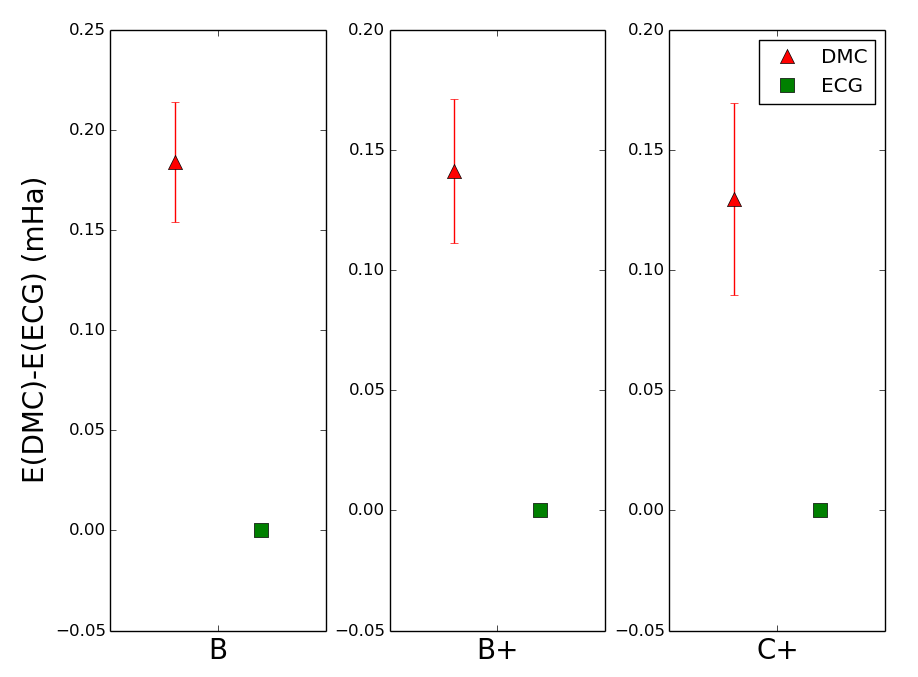
\includegraphics[scale=.4]{Figures/atom-ECG}
\caption{FN-DMC ground state energies for $\text{Be}^+$, Be, $\text{B}^+$, B, $\text{C}^+$ relative to ECG references~\cite{Stanke_Be,Puchalski_Be+,Bubin_BeH_noBO,Bubin_B,Bubin_B+,Bubin_C+} for either clamped-ion or non-adiabatic calculations. These relative energies provide an estimate for the fixed-node error in the electronic and electron-ion wave functions respectively.\label{fig:atom-ECG}}
\end{figure}

As an illustration of the high quality QMC techniques used in this work, we compare our adiabatic atomic results with a recent QMC benchmark study~\cite{Seth_Bench}. The clamped-ion ground state FN-DMC energies consistently agree across all systems (except for O$^{+}$), within error bars. This is an interesting coincidence since we used a different approach in optimizing our wave functions. In particular our large ($\sim$ 1000 CSF) multi-determinant expansions can be compared with the approach used by Seth {\it et al.}~\cite{Seth_Bench}, which relies on moderately-sized multi-determinant expansions ($\sim$ 100 CSF) with a backflow transformation. 

For the atomic systems, there are five ECG calculations of non-adiabatic ground state energies we can use as benchmarks. The non-adiabatic ground-state energies for Be, $\text{Be}^+$, B, $\text{B}^+$ and $\text{C}^+$ are in agreement with ECG results within 0.3 mHa as shown in Figure \ref{fig:atom-ECG}. In Figure \ref{fig:atom-ECG}, the error bars for the reference ECG results are absorbed into the DMC error bars for clarity. Assuming the ECG results are converged to the exact ground-state energies in both the clamped-ion and non-adiabatic cases, the difference between our clamped-ion DMC ground-state and ECG reference is the amount of fixed-node error present in our electronic wave functions, while its non-adiabatic counterpart is the fixed-node error for the electron-ion wave function. We see that the fixed-node error in the electron-ion wave functions can be larger than that in the electronic wave function at the sub-mHa level. Since the dragged-node approximation does not change the quality of nodes for atoms and ions and the ground-state ionic wave function is nodeless, the additional fixed-node error in the electron-ion wave function indicates that nuclear-electron correlation can non-trivially modify the nodes of the electronic wave function.

\begin{figure}[h]
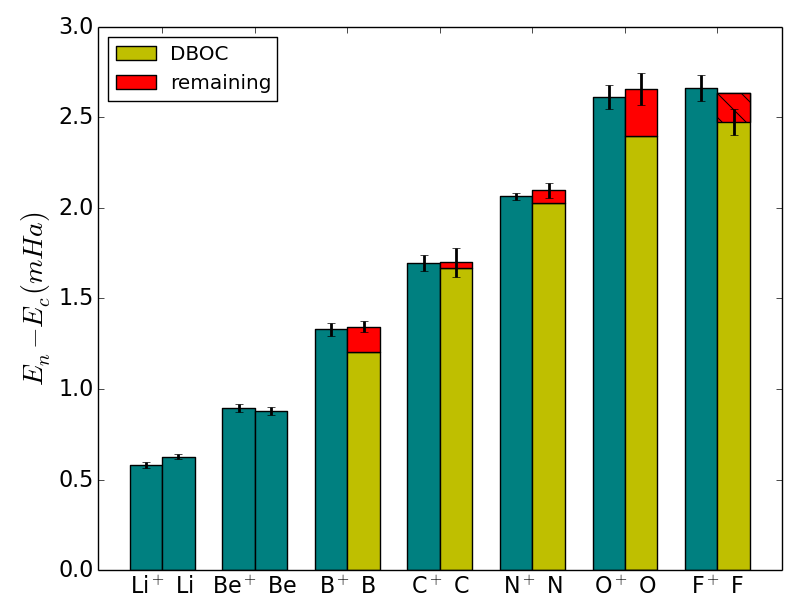
\includegraphics[scale=.37]{Figures/atom-nad-ad}
\caption{Non-adiabatic contribution to ground state energies of atoms and ions calculated with FN-DMC. $E_n^{DMC}$ denotes the non-adiabatic ground state energy and $E_c^{DMC}$ the clamped-ion ground state energy. Non-adiabatic contribution is partitioned into DBOC and the remaining correction whenever data is available. A hatched bar indicates the contribution is negative. \label{fig:atom-nad-ad}} %Non-adiabatic contribution shows very little dependence with the ionized state.
\end{figure}

\begin{figure}[h]
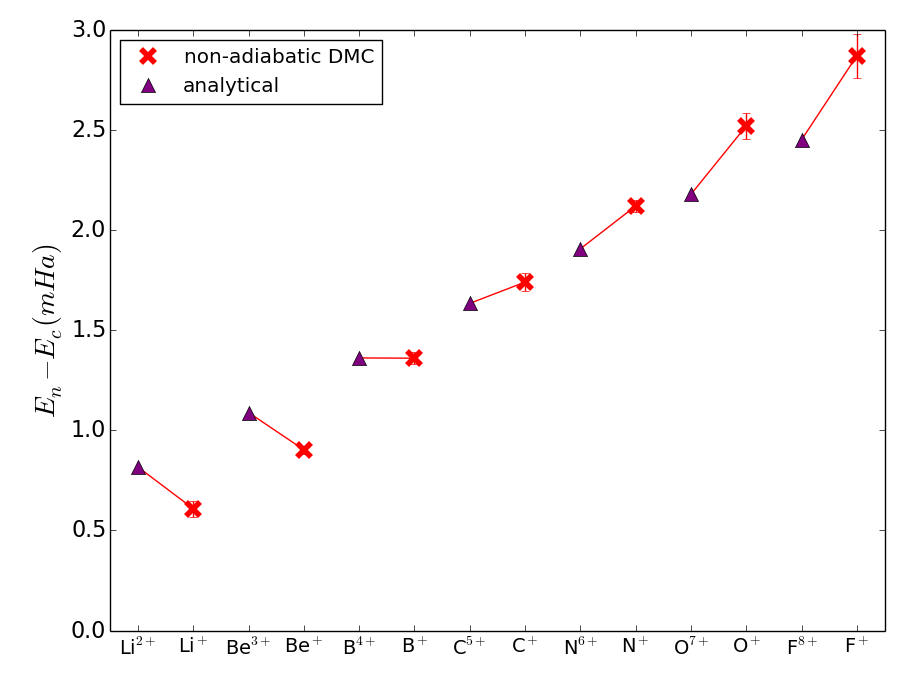
\includegraphics[scale=.4]{Figures/analytical}
\caption{Non-adiabatic contribution to ground state energies of ions and their hydrogen-like atoms calculated with FN-DMC and analytically. $E_n$ denotes the non-adiabatic ground state energy and $E_c$ the clamped-ion ground state energy. \label{fig:analytical}}
\end{figure}

In Figure \ref{fig:atom-nad-ad}, we demonstrate the amount of non-adiabatic contribution to ground-state energies in atoms and ions calculated as the difference between the non-adiabatic and clamped-ion ground-state energies. Non-adiabatic contribution includes DBOC as well as any other contribution arising from the difference between the true wave function and the BO product ansatz. As shown in Figure \ref{fig:atom-nad-ad}, the amount of non-adiabatic contribution is always positive and increases with atomic number but stays relatively constant between the neutral and cationic species. This observation suggests that almost all of the non-adiabatic contribution can be attributed to the kinetic energy of the nucleus. Due to interaction with the electrons, the nucleus is effectively confined, which gives rise to a given amount of kinetic energy. This kinetic energy is closely related to the charge and mass of the nucleus but is less sensitive to the number of electrons in the system. This point is further illustrated by comparing the non-adiabatic contributions in the cations with their corresponding hydrogen-like atoms as shown in Figure \ref{fig:analytical}. The non-adiabatic contributions in the hydrogen-like atoms can be obtained analytically by using reduced mass. The result in Hartree atomic units is
\begin{align}
E_n-E_c=\frac{Z^2}{2}(1-\mu)
\end{align}
where $\mu=\frac{M}{M+1}$ is the reduced mass of the hydrogen-like atom and $M$,$Z$ are the the mass and atomic number of the nucleus respectively. We see in Figure \ref{fig:analytical} that even when going from 1 electron to 9 electrons in the case of $F$, the total non-adiabatic energy only changes by 0.5 mHa (17\%). It is also interesting to note that for $\text{Li}^{2+}$ and $\text{Be}^{3+}$, the addition of electrons decreases the overall non-adiabatic contribution whereas for $\text{C}^{5+}$ and heavier nuclei, the addition of electrons increase the it.

% This observation suggests that for atomic systems, the non-adiabatic coupling between electrons and the nucleus motion is small.
% For atoms and ions, DBOC physically describes the effective confinement of the nucleus due to coupling between the electronic and nuclear motions. This confinement will add a nuclear kinetic contribution to the camped-ion ground-state energy. Non-adiabatic effect encompasses the rest of the modifications to the electron-ion wave function due to electron-nuclear correlation.

The ionization potentials are reported in Table \ref{tab:ionization} and shown in Figure \ref{fig:ionization}. We combined the corrections from~\cite{Klopper_IP} and experimental data~\cite{NIST_Atoms} as reference instead of \cite{Davidson_Atoms} because the latter estimates ionization potentials in the infinite-nucleus-mass limit. However, as discussed in \cite{Seth_Bench}, the difference between the two references is small. Our clamped-ion results all lie within 1 mHa of the reference. In particular, whenever our result is statistically different from the reference, we underestimate the ionization potential. One explanation for this trend is that it is significantly more difficult to obtain a good wave function for the neutral than the cationic species of a given nucleus. Other QMC studies seem to experience similar difficulties \cite{Seth_Bench,Booth_FCIQMC,Brown_Bench}. It is interesting to note that even though the ground-state energy of an atom can differ significantly from the clamped-ion to the non-adiabatic calculation (as much as 3 mHa for $\text{F}^+$). The ionization potentials calculated with and without the Born-Oppenheimer approximation are statistically indistinguishable except for O and F, where the non-adiabatic effects on the ionization energies are 0.26(11)mHa and 0.49(12)mHa respectively. It is possible that these differences are not physical but rather an artifact of the drag-node approximation as they are comparable to the fixed-node error shown in Figure \ref{fig:atom-ECG}. The estimated DBOC for the ionization potentials of O and F in~\cite{Klopper_IP} are both two orders of magnitude smaller than our error bars, which further suggests that the clamped-ion and non-adiabatic predictions of the ionization potentials should not be different at the sub-mHa level.

\begin{figure}
\centering
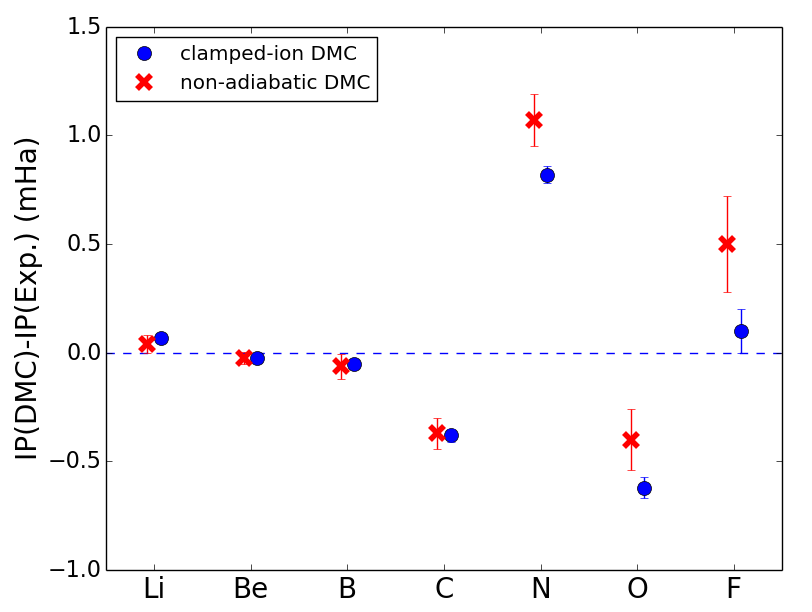
\includegraphics[scale=.4]{Figures/ionization}
\caption{Calculated ionization energies relative to experimental data. The calculated energies are all within 1 mHa of experiment. \label{fig:ionization}}
\end{figure}

\subsection{Hydrides}

\begin{table*}[t!]
\setlength{\extrarowheight}{1pt}
\begin{threeparttable}
\caption{Ground-state energies and atomization energies: fixed-node DMC results of this work for all first row hydrides with and without the Born-Oppenheimer approximation. The rows marked with bolded \textbf{FN-DMC} are our non-adiabatic results. All atomization energies are all estimated for 0K. $D_o$ includes zero-point energy contribution while $D_e$ does not. Energies are given in units of Hartree. \label{tab:atomization}}
\begin{tabular}
% siunitx setup
{
 l
 S[table-format=1.6]
 S[table-format=4.6]
 S[table-format=4.6]
 S[table-format=4.6]
 S[table-format=4.6]
 S[table-format=4.6]
 S[table-format=4.6]
}

\hline\hline
\multicolumn{1}{c}{Molecule} & 
\multicolumn{1}{c}{LiH$(^1\Sigma^+)$} &
\multicolumn{1}{c}{BeH$(^2\Sigma^+)$} &
\multicolumn{1}{c}{BH$(^1\Sigma^+)$} &
\multicolumn{1}{c}{CH$(^2\Pi)$} &
\multicolumn{1}{c}{OH$(^2\Pi)$} &
\multicolumn{1}{c}{HF$(^1\Sigma^+)$} \\ 
\hline
\multicolumn{1}{c}{} & 
\multicolumn{1}{c}{} &
\multicolumn{1}{c}{} &
\multicolumn{1}{c}{clamped-nuclei} &
\multicolumn{1}{c}{} &
\multicolumn{1}{c}{} &
\multicolumn{1}{c}{} \\
FN-DMC & \text{-}8.070518(2) & \text{-}15.24793(2) & \text{-}25.28867(2) & \text{-}38.47801(4) & \text{-}75.7357(1) & \text{-}100.4552(1) \\
$E_{\text{ref}}$ \tnote{a} & \text{-}8.0705473 & \text{-}15.2483(4) & \text{-}25.2893(2) & \text{-}38.4792(2) & \text{-}75.7382(2) & \text{-}100.4600(3) \\
\multicolumn{1}{c}{} & 
\multicolumn{1}{c}{} &
\multicolumn{1}{c}{} &
\multicolumn{1}{c}{non-adiabatic} &
\multicolumn{1}{c}{} &
\multicolumn{1}{c}{} &
\multicolumn{1}{c}{} \\
\textbf{FN-DMC} & \text{-}8.06624(2) & \text{-}15.24194(4) & \text{-}25.28102(2) & \text{-}38.46721(3) & \text{-}75.72453(9) & \text{-}100.44315(7) \\
ECG \cite{Bubin_LiH_noBO,Bubin_BeH_noBO,Bubin_BH_noBO} & \text{-}8.0664371(15) & \text{-}15.24203(10) & \text{-}25.2803(10) & N/A & N/A & N/A \\
\hline

\multicolumn{1}{c}{} & 
\multicolumn{1}{c}{} &
\multicolumn{1}{c}{} &
\multicolumn{1}{c}{clamped-nuclei} &
\multicolumn{1}{c}{} &
\multicolumn{1}{c}{} &
\multicolumn{1}{c}{} \\
$D_e$ (this work) & 0.09246(1) & 0.08062(2) & 0.13493(3) & 0.13353(5) & 0.1699(1) & 0.2234(1) \\
$D_e$ Feller \tnote{b} & 0.09262(5) & 0.0809(4) & 0.1354(2) & 0.1342(2) & 0.1709(2) & 0.2258(3) \\
\multicolumn{1}{c}{} & 
\multicolumn{1}{c}{} &
\multicolumn{1}{c}{} &
\multicolumn{1}{c}{non-adiabatic} &
\multicolumn{1}{c}{} &
\multicolumn{1}{c}{} &
\multicolumn{1}{c}{} \\
$D_o$ (this work) & 0.08908(4)  & 0.07578(4)  & 0.12890(4) & 0.12480(9) & 0.1617(1) & 0.2141(1) \\
$D_o$ Feller \tnote{c} & 0.08940(5) & 0.0761(4) & 0.1299(2) & 0.1276(2) & 0.1622(2) & 0.2166(3)\\
$D_o$ Exp. \cite{CCCBDB,HH} & 0.08874(38) & 0.07475(4) & 0.1281(37)\tnote{d} & 0.1275(5) & 0.1622(1) & 0.2158(3) \\
\hline\hline
\end{tabular}
\begin{tablenotes}
\item[a] For LiH, ECG provides the best reference energy~\cite{Adamowicz_LiH}. For the rest of the systems, we combined the best clamped-ion atomic references in Table \ref{tab:ionization} and thermochemistry estimates of $D_e$ in this table to produce the reference ground-state energies.
\item[b] Best estimates for $D_e$ are calculated by subtracting the scalar relativistic, spin-orbit coupling and zero-point energy corrections from the reference $D_o$ in Table VI of Ref.~\cite{Feller_Corrections}.
\item[c] Here only the scalar relativistic and spin-orbit coupling corrections are subtracted.
\item[d] The atomization energy for BeH in Ref.~\cite{CCCBDB} disagrees with previous high level theoretical benchmarks~\cite{Feller_Corrections,Bubin_BeH_noBO}, thus we use Ref.~\cite{HH} instead.
\end{tablenotes}
\end{threeparttable}
\end{table*}

The clamped-nuclei ground-state energies for LiH, BeH and BH are on par with the best available quantum chemistry references~\cite{Adamowicz_LiH,Koput_BeH,Miliordos_BH}. The non-adiabatic energies are in agreement with the ECG results for LiH and BeH to within 0.5 mHa as shown in Figure \ref{fig:dia-ECG}. For small systems, ECG results are typically orders of magnitude more accurate than the best QMC and other quantum chemistry calculations. However, with BH being one of the largest ECG simulations performed, the QMC result is actually lower in energy, in this case by 1 mHa. For the larger systems CH, OH, and HF, there are no explicit simulations we can compare against, and we combine semi-empirical~\cite{Davidson_Atoms} and thermochemistry results~\cite{Feller_Corrections} for comparison.

To estimate the non-adiabatic contribution to the ground-state energy of a hydride, we need to calculate the difference between a non-adiabatic and an adiabatic calculation. To produce adiabatic references we add the zero-point energies estimated in~\cite{Feller_Corrections} to our clamped-nuclei energies as exact corrections. The results are shown in Figure \ref{fig:dia-nad-ad}. The amount of non-adiabatic contribution for the hydrides investigated all fall in the range of a few mHa and seem to peak for CH and HF. However, it is likely that the actual amount of non-adiabatic energies are smaller than what is being shown in Figure \ref{fig:dia-nad-ad}, as the predicted atomization energies for CH and HF agree less well with experiments than their adiabatic counterparts.

\begin{figure}[h]
\centering
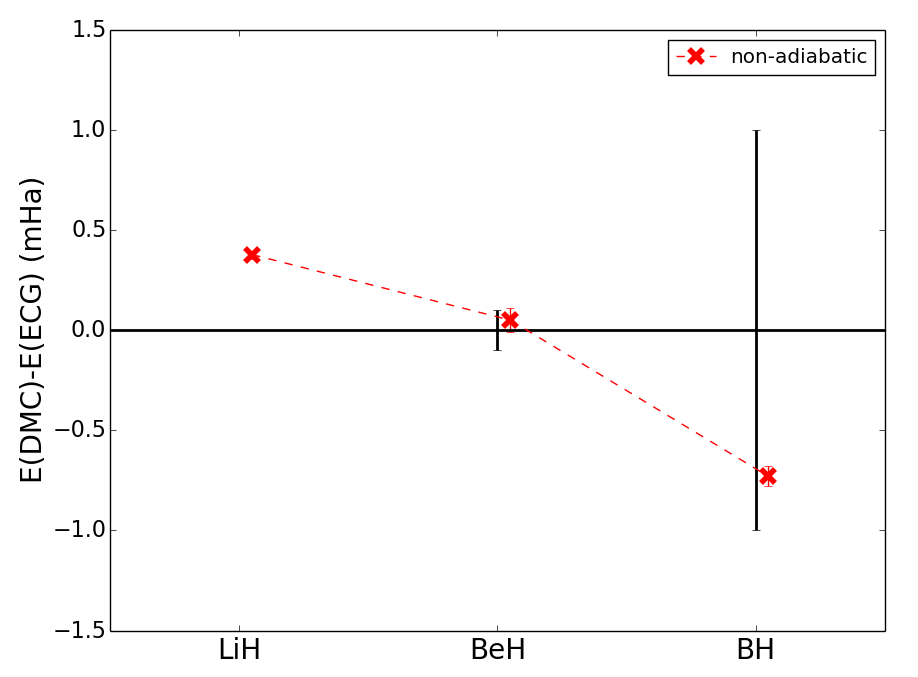
\includegraphics[scale=.37]{Figures/dia-ECG}
\caption{Non-adiabatic FN-DMC ground-state energies of LiH, BeH and BH relative to ECG references. The errorbars for the non-adiabatic ECG references are shown as thick dark lines and the errorbars for the FN-DMC calculations are comparible to the size of the markers. \label{fig:dia-ECG}}
\end{figure}

\begin{figure}[h]
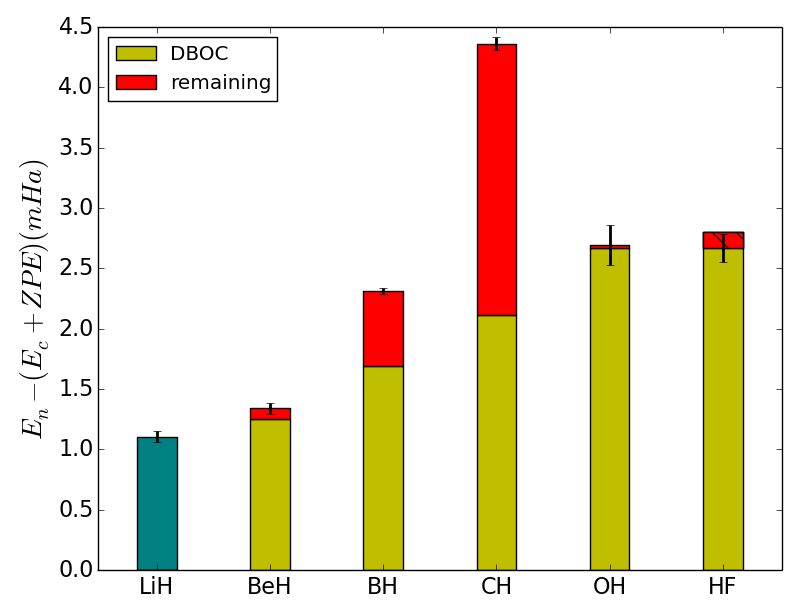
\includegraphics[scale=.37]{Figures/dia-nad-ad}
\caption{Non-adiabatic contribution to the ground-state energies in hydrides. The adiabatic reference energies are calculated by adding zero-point contributions from \cite{Feller_Corrections} to our clamped-nuclei results. A hatched bar indicates the contribution is negative. \label{fig:dia-nad-ad}}
\end{figure}

For the LiH molecule we are also interested in calculating the electron affinity for comparison to ECG results. We calculated the ground state energy of LiH$^-$ to be $-8.08220(2)$~Ha for the case of clamped nuclei.  With non-adiabatic effects included our result is  $-8.07811(3)$~Ha. Our non-adiabatic result is in good agreement with a previous ECG study \cite{Bubin_LiH_noBO}, which reported a value of $-8.07856887$~Ha. We report an electron affinity of $0.01191(4)$~Ha, which can be compared to the ECG prediction of $0.012132(2)$~Ha and agrees with experiment, $0.0126(4)$~Ha. \footnote{We note that LiH ground state energies which we compare against are mislabeled in Ref.\cite{Bubin_LiH_noBO}, with $\text{LiH}^-$ and LiD being switched.}

\begin{figure}[h]
\centering
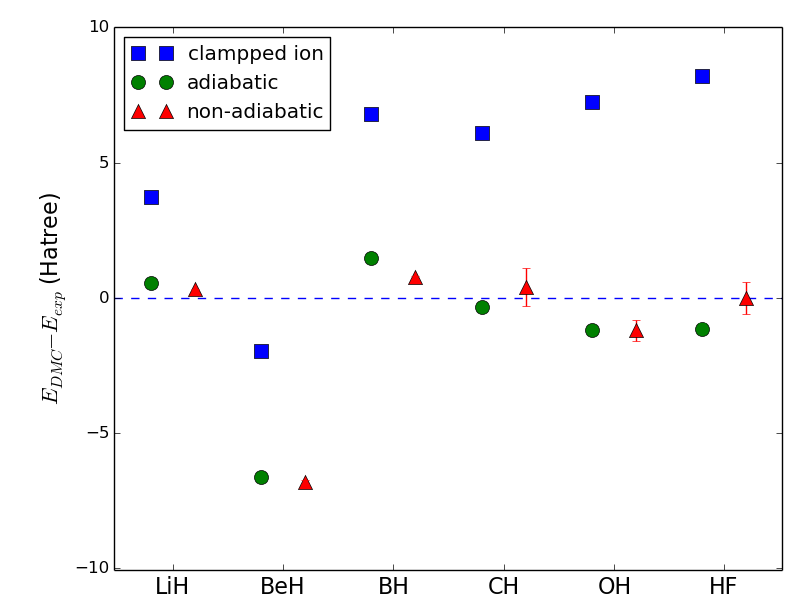
\includegraphics[scale=.4]{Figures/atomization}
\caption{Atomization energies of first row hydrides obtained with FN-DMC relative to experimental data. The adiabatic results are estimated by adding zero-point energies from \cite{Feller_Corrections} to the clamped nuclei energies as exact corrections. \label{fig:atomization}}
\end{figure}

The atomization energy of the diatomic systems are reported in Table \ref{tab:atomization} and shown in Figure \ref{fig:atomization}. There are high quality thermochemistry benchmark results to which we can compare~\cite{Feller_Corrections}. To compare against the thermochemistry benchmark results, we take the reference energies from the last column of Table VI of Ref.~\cite{Feller_Corrections} and subtract the corrections in the $\Delta E_{SR}$ (scalar relativistic) and SO (spin-orbit coupling) columns for comparison with our non-adiabatic energies. For the comparison with our adiabatic energies, we further subtract the DBOC (diagonal Born-Oppenheimer correction) and ZPE (zero-point energy) corrections. Corrections from spin-orbit coupling and relativistic effects are not used, as they are not included in our Hamiltonian. Our biggest errors appear to occur for BeH and CH. For the case of BeH we agree with accuracy higher than 1 mHa with both the ECG results~\cite{Bubin_BeH_noBO} and semi-empirical benchmark~\cite{Feller_Corrections,Davidson_Atoms}. In particular, the ECG results are converged to more digits than the experimental error bar, and it is likely the experimental reference has errors on the order of 5 mHa. For the case of CH, our error is on the order of 3 mHa, which can be due to the dragged-node approximation. 

\section{Conclusion}
We calculated the ground-state energies of first row atoms and their corresponding ions and hydrides to an accuracy of $0.1$ mHa for all but the largest systems with and without the Born-Oppenheimer assumption. We found the ionization energies of the atoms to be relatively independent of the adiabatic approximation, whereas the atomization energies are affected at the sub-mHa level. We provided benchmark data for the amount of non-adiabatic energy contribution for all systems studied. % and note that DBOC likely dominates the non-adiabatic energy in atoms and ions.

These calculations also verified the validity of our wave function ansatz, namely it does indeed produce a high quality electron-ion trial wave function from a good electron wave function. This technique also has the potential to solve interesting larger-scale problems due to its ease of implementation as well as the polynomial scaling in computational time with respect to the number of electrons.  This technique can be generalized quite easily to deal with larger systems.

\section{Acknowledgment}
The authors would like to thank Mike Pak, Kurt Brorsen, Katharina Doblhoff-Dier and Brian Busemeyer for useful discussions. The authors would also like to thank Prof. Willem Klopper for providing the DBOC references for the atoms and ions and Prof. David Feller for providing the DBOC data for the hydrides. This work was supported by the U.S. Department of Energy grant No. 1-485267-244000-191100 as part of the Scientific Discovery through Advanced Computing (SciDAC) program. We used the Extreme Science and Engineering Discovery Environment (XSEDE), which is supported by the National Science Foundation Grant No. OCI-1053575 and resources of the Oak Ridge Leadership Computing Facility (OLCF) at the Oak Ridge National Laboratory, which is supported by the Office of Science of the U.S. Department of Energy under Contract No. DE-AC05-00OR22725.

\bibliography{ref}
\end{document}
